Model návrhu dále \textbf{upřesňuje model analýzy ve světle skutečného implementačního prostředí}. Model návrhu tak představuje \textbf{druhou fázi} vývoje softwaru. Jde o abstrakci zdrojového kódu, která bude sloužit jako hlavní dokument programátorům v další implementační fázi.

\subsection{Návrh a jeho cíle}
Pojem implementační prostředí v podstatě vyjadřuje \textbf{možnost namapovat navržené softwarové komponenty} obsažené v modelu analýzy na architekturu systému určeného k provozu vyvíjené aplikace \textbf{s maximálním možným využitím služeb již existujících softwarových komponent}. Postup včlenění implementačního prostředí do vyvíjené aplikace je dán následující posloupností činností:
\begin{enumerate}
\item Definice \textbf{systémové architektury}.
\item Identifikace \textbf{návrhových vzorů} a možnosti znovupoužití tzv. rámcových řešení.
\item Definice softwarových komponent a jejich \textbf{znovupoužití}.
\end{enumerate}
V této fázi se uplatňují následující diagramy:

\begin{itemize}
\item \textbf{Diagram tříd} - specifikuje \textbf{množinu tříd, rozhraní a jejich vzájemné vztahy}. Tyto diagramy slouží k vyjádření \textbf{statického} pohledu na systém.
\item \textbf{Sekvenční diagram} - popisuje \textbf{interakce mezi objekty} z hlediska jejich \textbf{časového} uspořádaní.
\item \textbf{Diagram spolupráce} - je obdobně jako sekvenční diagram zaměřen na \textbf{interakce}, ale {z pohledu strukturální organizace objektů}. Jinými slovy není primárním aspektem časová posloupnost posílaných zpráv, ale \textbf{topologie rozmístění objektů}.
\item \textbf{Stavový diagram} - dokumentuje \textbf{životní cyklus objektu} dané třídy a stavy, ve kterých se může nacházet.
\item \textbf{Diagram nasazení} - popisuje \textbf{konfiguraci} (topologii) \textbf{technických prostředků} umožňující běh vlastního softwarového systému (rozmístění HW a SW).
\end{itemize}

\begin{figure}[H]
	\centering
	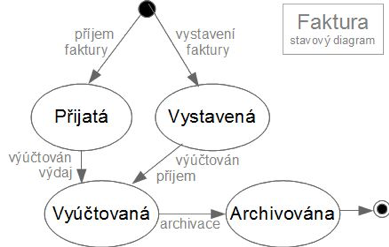
\includegraphics[width=.4\textwidth]{assets/diag_stavovy.png}
\end{figure}
\begin{figure}
	\centering
	\begin{minipage}{.5\textwidth}
		\centering
		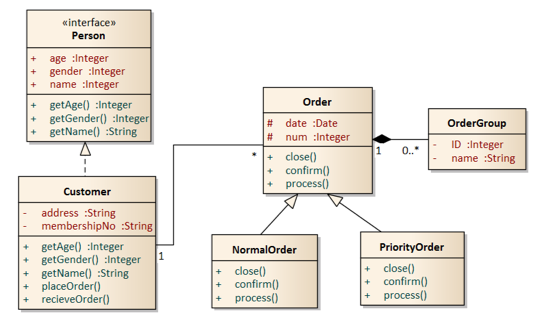
\includegraphics[width=.95\linewidth]{assets/diag_tridni.png}
	\end{minipage}%
	\begin{minipage}{.5\textwidth}
		\centering
		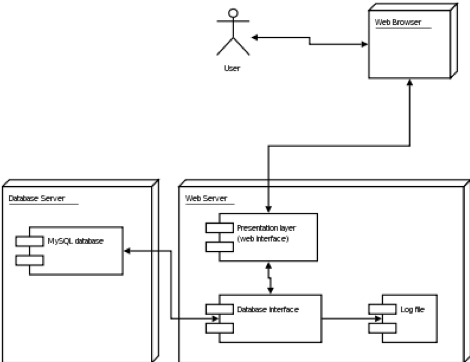
\includegraphics[width=.95\linewidth]{assets/diag_nasazeni.png}
	\end{minipage}
\end{figure}

\subsection{Návrhové vzory - členění}
Návrhové vzory jsou metodiky (šablony) pro \textbf{řešení různých problému}, se kterými se vývojář může setkat. Objektově orientované návrhové vzory typicky ukazují \textbf{vztahy} a \textbf{interakce mezi třídami a objekty}, aniž by určovaly implementaci konkrétní třídy. Dělí se do tří základních skupin:
\begin{itemize}
\item \textbf{Creational Patterns (vytvářející)} - určené k řešení problému vytváření instancí tříd cestou delegace této funkce na speciálně k tomuto účelu navržené třídy. Většinou se jedná o dynamická rozhodnutí učiněná za běhu programu.
\item \textbf{Structural Patterns (strukturální)} - představují skupinu návrhových vzorů zaměřujících se na možnosti uspořádání jednotlivých objektů a jejich tříd nebo komponent v systému. Snahou je zpřehlednit systém a využít možností strukturalizace kódu.
\item \textbf{Behavioral Patterns (chování)} - zajímají se o chování systému. Mohou být založeny na třídách nebo objektech. U tříd využívají při návrhu řešení především principu dědičnosti. V druhém přístupu je \textbf{řešena spolupráce mezi objekty a skupinami objektů}, která zajišťuje dosažení požadovaného výsledku.
\end{itemize}

\subsubsection{Creational patterns (Vzory týkající se tvorby objektů)}
\begin{itemize}
	\item \textbf{Abstract Factory (Abstraktní továrna)} - Definuje rozhraní pro vytváření rodin objektů, které jsou na sobě závislé nebo spolu nějak souvisí bez určení konkrétní třídy. Klient je odstíněn od vytváření konkrétních instancí objektů.
	\item \textbf{Factory Method (Tovární metoda)} - Definuje rozhraní pro vytváření objektu, které nechává potomky rozhodnout o tom, jaký objekt bude fakticky vytvořen. *Tovární metoda nechává třídy přenést vytváření na potomky.
	\item \textbf{Builder (Stavitel)} - Odděluje tvorbu komplexu objektů od jejich reprezentace tak, aby stejný proces tvorby mohl být použit i pro jiné reprezentace.
	\item \textbf{Singleton (Jedináček)} - Zajišťuje, že daná třída má pouze jednu instanci (využívá se privátních konstruktorů a samotná třída ve statické proměnné uchovává danou instanci).
	\item \textbf{Prototype (Prototyp, Klon)} - Specifikuje druh objektů, které se mají vytvořit použitím prototypového objektu. Nové objekty se vytváří kopírováním tohoto prototypového objektu.
\end{itemize}

\subsubsection{Structural Patterns (Vzory týkající se struktury programu)}
\begin{itemize}
	\item \textbf{Adapter (Adaptér)} - Potřebujete-li, aby spolu pracovaly dvě třídy, které nemají kompatibilní rozhraní. Adaptér převádí rozhraní jedné třídy na rozhraní druhé třídy.
	\item \textbf{Bridge (Most)} - Oddělí abstrakci od implementace, tak aby se tyto dvě mohly libovolně lišit.
	\item \textbf{Composite (Kompozit, Strom, Složenina)} - Komponuje objekty do stromové struktury a umožňuje klientovi pracovat s jednotlivými i se složenými objekty stejným způsobem.
	\item \textbf{Decorator (Dekorátor)} - Dekorátor se vytváří za účelem změny instancí tříd bez nutnosti vytvoření nových odvozených tříd, jelikož pouze dynamicky připojuje další funkčnosti k objektu. Nový objekt si zachovává původní rozhraní.
	\item \textbf{Facade (Fasáda)} - Nabízí jednotné rozhraní k sadě rozhraní v podsystému. Definuje rozhraní vyšší úrovně, které zjednodušuje použití podsystému.
	\item \textbf{Flyweight (Muší váha)} - Je vhodná pro použití v případě, že máte příliš mnoho malých objektů, které jsou si velmi podobné.
	\item \textbf{Proxy} - Nabízí náhradu nebo zástupný objekt za nějaký jiný pro kontrolu přístupu k danému objektu.
\end{itemize}

\subsubsection{Behavioral Patterns (Vzory týkající se chování)}
\begin{itemize}
	\item \textbf{Observer (Pozorovatel)} - V případě, kdy je na jednom objektu závislých mnoho dalších objektů, poskytne vám tento vzor způsob, jak všem dát vědět, když se něco změní. Observer je možné použít v situaci, kdy je definována závislost jednoho objektu na druhém. Závislost ve smyslu propagace změny nezávislého objektu závislým objektům (pozorovatelům). Nezávislý objekt musí informovat závislé objekty o \textbf{událostech}, které je mohou ovlivnit.
	\item \textbf{Command (Příkaz)} - Zapouzdřete požadavek jako objekt a tím umožněte parametrizovat klienty s různými požadavky, frontami nebo požadavky na log a podporujte operace, které jdou vzít zpět.
	\item \textbf{Interpreter (Interpret)} - Vytváří jazyk, což znamená definování gramatických pravidel a určení způsobu, jak vzniklý jazyk interpretovat.
	\item \textbf{State (Stav)} - Umožňuje objektu měnit své chování, pokud se změní jeho vnitřní stav. Objekt se tváří, jako kdyby se stal instancí jiné třídy.
	\item \textbf{Strategy (Strategie)} - Zapouzdřuje nějaký druh algoritmů nebo objektů, které se mají měnit, tak aby byly pro klienta zaměnitelné.
	\item \textbf{Chain of responsibility (Zřetězení zodpovědnosti)} - Řeší jak zaslat požadavek bez přesného vymezení objektu, který jej zpracuje.
	\item \textbf{Visitor (Návštěvník)} - Reprezentuje operaci, která by měla být provedena na elementech objektové struktury. Visitor vám umožní definovat nové operace beze změny tříd elementů na kterých pracuje.
	\item \textbf{Iterator (Iterátor)} - Řeší problém, jak se pohybovat mezi prvky, které jsou sekvenčně uspořádány, bez znalosti implementace jednotlivých prvků posloupnosti.
	\item \textbf{Mediator (Prostředník)} - Umožňuje zajistit komunikaci mezi dvěma komponentami programu, aniž by byly v přímé interakci a tím musely přesně znát poskytované metody.
	\item \textbf{Memento (Memento)} - Bez porušování zapouzdření zachyťte a uložte do externího objektu interní stav objektu tak, aby ten objekt mohl být do tohoto stavu kdykoliv později vrácen.
	\item \textbf{Template method (Šablonová metoda)} - Definuje kostru toho, jak nějaký algoritmus funguje, s tím, že některé kroky nechává na potomcích. Umožňuje tak potomkům upravit určité kroky algoritmu bez toho, aby mohli měnit strukturu algoritmu.
\end{itemize}
